\documentclass[a4paper,11pt]{article}
\usepackage[utf8]{inputenc}
\usepackage[T1]{fontenc}
\usepackage{lmodern}
\usepackage[margin=2.5cm]{geometry}
\usepackage{graphicx}
\usepackage{booktabs}
\usepackage{array}
\usepackage{float}
\usepackage{seqsplit}

\title{Trabalho Prático 2 --- Reconhecimento de Produtos\\por Correspondência de Características Locais}
\author{Bruno Ribeiro \and Monique Machado}
\date{}

\begin{document}
\maketitle

\section*{1. Templates utilizados}

Um template por classe, recortado manualmente da região do rótulo com o nome do produto,
a partir de uma imagem do conjunto \texttt{Train\_and\_Validation} de cada classe.

\begin{table}[H]
\centering
\small
\begin{tabular}{@{}p{2.6cm} p{3.6cm} p{7.0cm}@{}}
\toprule
\textbf{Produto} & \textbf{Imagem utilizada} & \textbf{Justificativa} \\
\midrule
Meio das Asas                        & \scriptsize\ttfamily\seqsplit{meio-da-assa-gold.jpg}               & \normalsize Texto em alto contraste, sem sobreposição de outros elementos do rótulo. \\
Coxinhas das Asas                    & \scriptsize\ttfamily\seqsplit{coxinha-das-asas-gold.jpg}           & \normalsize Recorte nítido do nome do produto, bordas do texto bem definidas. \\
Filé de Peito                        & \scriptsize\ttfamily\seqsplit{file-de-peito-gold.jpg}              & \normalsize Texto curto e bem preservado, boa nitidez e contraste com o fundo. \\
Coração                              & \scriptsize\ttfamily\seqsplit{coracao-gold.jpg}                    & \normalsize Palavra única de alto potencial discriminativo, sem elementos repetidos entre classes. \\
Moela                                & \scriptsize\ttfamily\seqsplit{moela-gold.jpg}                      & \normalsize Palavra curta e exclusiva dessa classe, baixa chance de correspondência espúria. \\
Filé de Coxas e Sobrecoxas com Pele  & \scriptsize\ttfamily\seqsplit{file\_de\_coxas\_e\_sobrecoxas-gold.jpg} & \normalsize Região com maior quantidade de detalhes (duas linhas de texto), maior número de pontos de interesse extraídos. \\
Coxas e Sobrecoxas                   & \scriptsize\ttfamily\seqsplit{coxas\_e\_sobrecoxas-gold.jpg}       & \normalsize Texto em duas linhas bem preservado, boa nitidez e contraste. \\
\bottomrule
\end{tabular}
\caption{Templates utilizados, um por classe (embalagens tipo bandeja).}
\end{table}

\section*{2. Parâmetros do algoritmo}

\textbf{Descritor local:} SIFT (\texttt{cv2.SIFT\_create}), com opção de troca para ORB via configuração.

\textbf{Casamento (matching):} \texttt{cv2.FlannBasedMatcher} (FLANN, permitido pelo enunciado),
com teste de razão de Lowe aplicado nos dois sentidos (cross-check) e verificação geométrica por
RANSAC (transformação afim), para descartar correspondências espúrias em elementos repetidos entre
rótulos (marca, "CONGELADO", tabela de peso).

\begin{table}[H]
\centering
\small
\begin{tabular}{@{}p{11.5cm} r@{}}
\toprule
\textbf{Parâmetro} & \textbf{Valor} \\
\midrule
Descritor                                    & SIFT \\
Razão de Lowe (\texttt{ratio\_test})         & 0,75 \\
Mínimo de matches para tentar RANSAC (\texttt{ransac\_min\_matches}) & 6 \\
Limiar de resíduo do RANSAC (\texttt{ransac\_residual\_px})         & 8,0 px \\
Mínimo de keypoints para extrair features (\texttt{min\_keypoints}) & 8 \\
\textbf{Limiar de correspondências válidas} (\texttt{min\_match\_frac}) & \textbf{0,08} \\
\bottomrule
\end{tabular}
\caption{Parâmetros fixos do algoritmo.}
\end{table}

\texttt{min\_match\_frac} é o único parâmetro de calibração exigido pelo enunciado: a fração de
correspondências válidas (inliers geométricos) sobre o número de pontos de interesse do template.
O template com maior fração vence a classificação do segmento, desde que essa fração atinja o
limiar; caso contrário, o segmento é reportado como \emph{não identificado} em vez de arriscar uma
classe errada.

\subsection*{Histórico de calibração (varredura de \texttt{min\_match\_frac})}

\begin{table}[H]
\centering
\small
\begin{tabular}{@{}*{5}{>{\centering\arraybackslash}p{2.5cm}}@{}}
\toprule
\textbf{min\_match\_frac} & \textbf{Acurácia (\%)} & \textbf{Não identificado} & \textbf{Falsos positivos} & \textbf{Taxa de FP (\%)} \\
\midrule
0,00 & 92,3 & 0   & 27  & 7,7 \\
0,02 & 92,0 & 5   & 23  & 6,6 \\
0,04 & 90,9 & 11  & 21  & 6,0 \\
0,06 & 88,0 & 27  & 15  & 4,3 \\
\textbf{0,08} & \textbf{83,4} & \textbf{48} & \textbf{10} & \textbf{2,9} \\
0,10 & 73,4 & 88  & 5   & 1,4 \\
0,12 & 62,9 & 127 & 3   & 0,9 \\
0,15 & 46,0 & 189 & 0   & 0,0 \\
0,20 & 22,0 & 273 & 0   & 0,0 \\
\bottomrule
\end{tabular}
\caption{Varredura do limiar de calibração sobre as 350 imagens avaliadas. O valor 0,08 foi
escolhido por manter a taxa de falsos positivos baixa (2,9\%) sem descartar recall demais,
priorizando minimizar falso positivo conforme pedido no enunciado.}
\end{table}

\section*{3. Resultados}

Avaliação sobre as 350 imagens de \texttt{crops-t1/} (7 classes bandeja, 50 imagens cada,
segmentos obtidos no T1 e corrigidos manualmente quando necessário), com
\texttt{min\_match\_frac = 0,08}.

\begin{table}[H]
\centering
\small
\begin{tabular}{@{}p{4.5cm} *{4}{>{\centering\arraybackslash}p{2.1cm}}@{}}
\toprule
\textbf{Produto} & \textbf{Total de imagens} & \textbf{Acertos} & \textbf{Não detectado} & \textbf{Falsos Positivos} \\
\midrule
Meio das Asas                        & 50  & 45  & 2  & 3  \\
Coxinhas das Asas                    & 50  & 32  & 17 & 1  \\
Filé de Peito                        & 50  & 50  & 0  & 0  \\
Coração                              & 50  & 50  & 0  & 0  \\
Moela                                & 50  & 45  & 5  & 0  \\
Filé de Coxas e Sobrecoxas com Pele  & 50  & 24  & 20 & 6  \\
Coxas e Sobrecoxas                   & 50  & 46  & 4  & 0  \\
\midrule
\textbf{Total}                       & \textbf{350} & \textbf{292} & \textbf{48} & \textbf{10} \\
\bottomrule
\end{tabular}
\caption{Resultado por classe. Acurácia global: 292/350 = 83,4\%. Falsos positivos: 10/350 = 2,9\%.}
\end{table}

\begin{figure}[H]
\centering
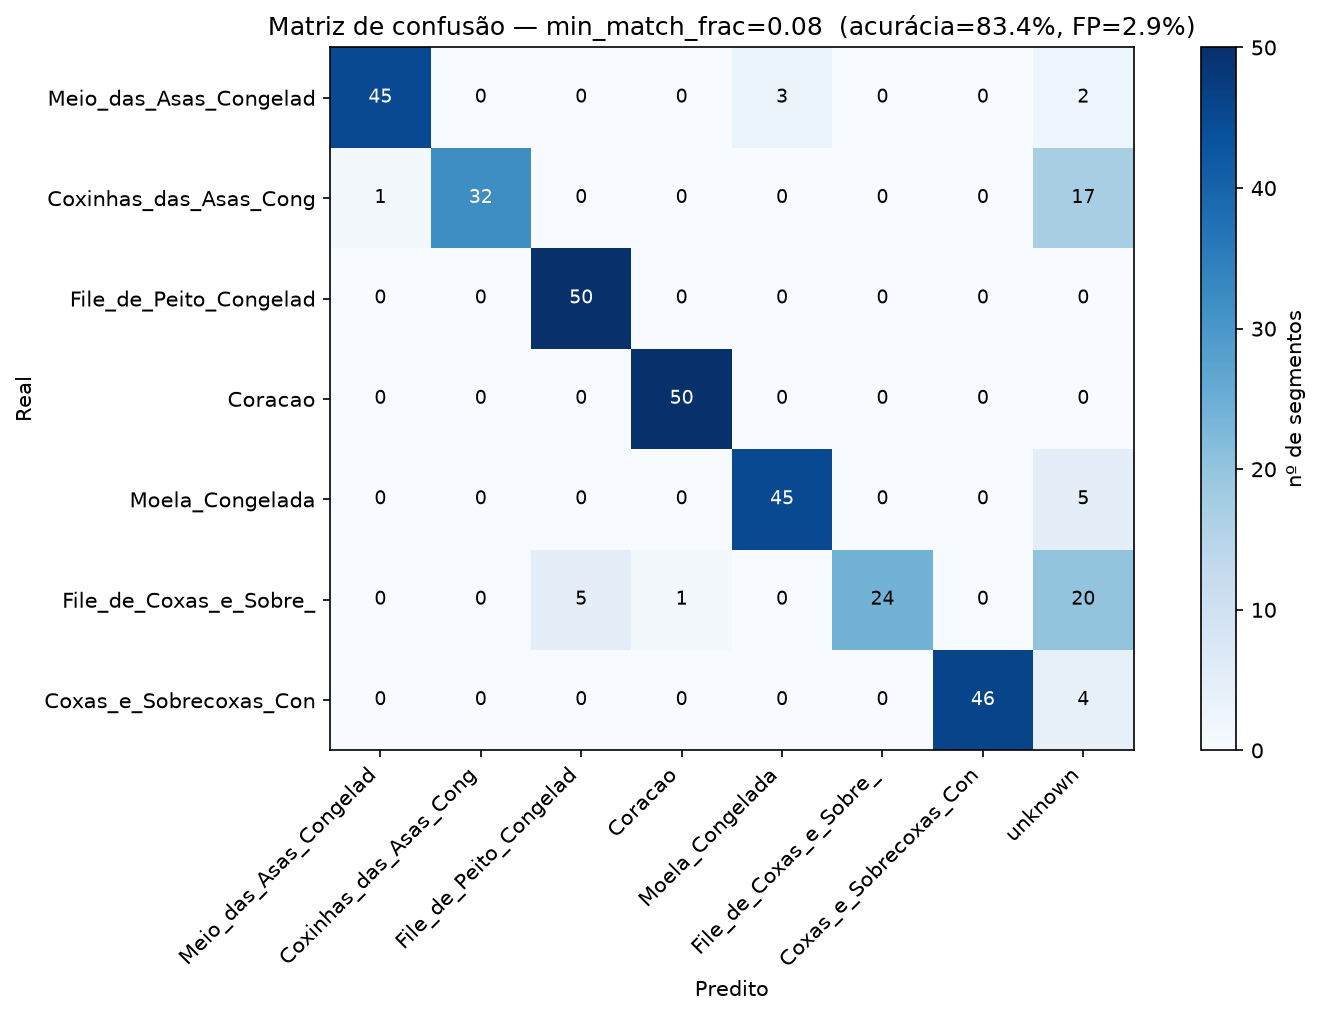
\includegraphics[width=\textwidth]{matriz_confusao_t2.png}
\caption{Matriz de confusão (linhas = classe real, colunas = classe predita) para
\texttt{min\_match\_frac = 0,08}. A diagonal principal mostra os acertos por classe; células
fora da diagonal (colunas 1--7) são falsos positivos (segmento classificado com o produto
errado); a última coluna, \emph{unknown}, conta os segmentos não identificados (score abaixo do
limiar de calibração). A escala de cor (barra à direita) indica o número de segmentos em cada
célula, de 0 (branco) a 50 (azul escuro).}
\end{figure}

\end{document}
